\documentclass[tikz,border=2pt]{standalone}
\usepackage{amsmath,amssymb}
\usepackage{tikz}

\begin{document}
% Disjoint sets have no element in common: the two regions do not overlap (A ∩ B = ∅).
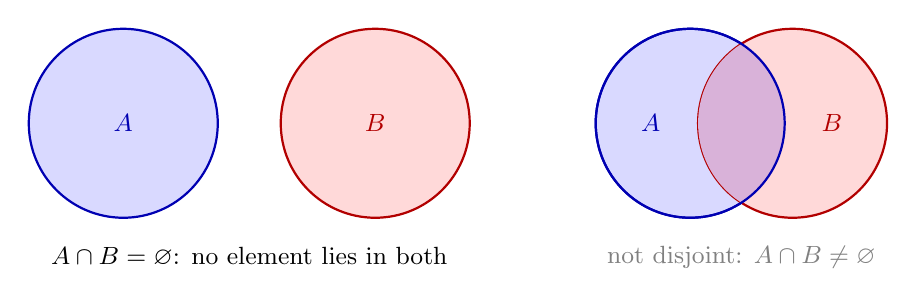
\begin{tikzpicture}[every node/.style={font=\small}]
	\draw[thick, blue!70!black, fill=blue!15] (0,0) circle (1.2);
	\draw[thick, red!70!black, fill=red!15] (3.2,0) circle (1.2);
	\node[blue!70!black] at (0,0) {$A$};
	\node[red!70!black] at (3.2,0) {$B$};
	\node at (1.6,-1.7) {$A\cap B=\varnothing$: no element lies in both};
	\begin{scope}[xshift=7.2cm]
		\draw[thick, blue!70!black, fill=blue!15] (0,0) circle (1.2);
		\draw[thick, red!70!black, fill=red!15] (1.3,0) circle (1.2);
		\begin{scope}
			\clip (0,0) circle (1.2);
			\fill[violet!30] (1.3,0) circle (1.2);
		\end{scope}
		\draw[thick, blue!70!black] (0,0) circle (1.2);
		\node[blue!70!black] at (-0.5,0) {$A$};
		\node[red!70!black] at (1.8,0) {$B$};
		\node[gray] at (0.65,-1.7) {not disjoint: $A\cap B\neq\varnothing$};
	\end{scope}
\end{tikzpicture}
\end{document}
